\documentclass[12pt, a4paper]{article}
\usepackage[T1]{fontenc} 
\usepackage[utf8]{inputenc}
\usepackage[english]{babel}
\usepackage{amsfonts}
\usepackage{amsmath}
\usepackage{graphicx}
\usepackage{listings}
\usepackage{xcolor}
\usepackage{tikz}
\usepackage{hyperref}
\usepackage{titlesec}
\usepackage[lmargin=2cm,rmargin=2cm,tmargin=3cm,bmargin=2cm]{geometry}

\usepackage{listings}

\lstloadlanguages{C,C++,csh,Java}

\definecolor{red}{rgb}{0.6,0,0} 
\definecolor{blue}{rgb}{0,0,0.6}
\definecolor{green}{rgb}{0,0.8,0}
\definecolor{cyan}{rgb}{0.0,0.6,0.6}
\definecolor{mygray}{rgb}{0.97, 0.97, 0.97}

\lstdefinelanguage{sharpc}{
language=csh,
basicstyle=\footnotesize\ttfamily,
% numbers=left,
% numberstyle=\tiny,
% numbersep=5pt,
tabsize=2,
extendedchars=true,
breaklines=true,
frame=b,
stringstyle=\color{red}\ttfamily,
showspaces=false,
showtabs=false,
xleftmargin=5pt,
framexleftmargin=5pt,
framexrightmargin=5pt,
framexbottommargin=4pt,
commentstyle=\color{green},
morecomment=[l]{//}, %use comment-line-style!
morecomment=[s]{/*}{*/}, %for multiline comments
showstringspaces=false,
morekeywords={ abstract, as, base, bool, 
break, byte, case, catch, 
char, checked, class, const, 
continue, decimal, default, delegate, 
do, double, else, enum, 
event, explicit, extern, false, 
finally, fixed, float, for, 
foreach, goto, if, implicit, 
in, int, interface, internal, 
is, lock, long, namespace, 
new, null, object, operator, 
out, override, params, private, 
protected, public, readonly, ref, 
return, sbyte, sealed, short, 
sizeof, stackalloc, static, string, 
struct, switch, this, throw, 
true, try, typeof, uint, 
ulong, unchecked, unsafe, ushort, 
using, using static, virtual, void, 
volatile, while,add, alias, ascending,
async, await, by,
descending, dynamic, equals,
from, get, global,
group, into, join,
let, nameof, on,
orderby, partial,
remove, select, set,
unmanaged, value, var,
when, where, yield},
keywordstyle=\color{blue},
identifierstyle=\color{black},
backgroundcolor=\color{mygray},
}

\lstdefinelanguage{XML}
{
	morestring=[b]",
	morestring=[s]{>}{<},
	morecomment=[s]{<?}{?>},
	stringstyle=\color{black},
	identifierstyle=\color{blue},
	keywordstyle=\color{cyan},
	morekeywords={xmlns,version,type}% list your attributes here
}


%tikz config
\usetikzlibrary{er,positioning}


\makeindex


% paragraph indent and line height
\setlength{\parindent}{0em}
\setlength{\parskip}{1em}
%\renewcommand{\baselinestretch}{1}

%section = new page
\pagenumbering{arabic}
\newcommand{\sectionbreak}{\clearpage}

% set default language for lstset
\lstset{language=sharpc}

\begin{document}
\title{Key learnings for this project}
\author{Pascal Lüscher}

\maketitle
\thispagestyle{empty}
\tableofcontents{}

\section{Entity Framework}

\subsection{Packages}
\begin{table}
\centering
	\begin{tabular}{|l l|}
		\hline
		Package & Description \\
		\hline \hline
		Npgsql.EntityFrameworkCore.PostgreSQL & For postgresql db access \\
		
		Microsoft.EntityFrameworkCore.Design & For migrations \\
		\hline
	\end{tabular}
\end{table}

When splitting the entity framework code into a separate project, the startup project and the context needs to be passed to the migrate command äöü

\begin{lstlisting}[language=bash]
dotnet ef migrations add NAME \
-o Data/Migrations \
--startup-project ../Isitar.DoenerOrder.Api/Isitar.DoenerOrder.Api.csproj \
--context AppIdentityDbContext
\end{lstlisting}

\subsection{CLI}

\begin{table}
\centering
	\begin{tabular}{|l l|}
		\hline
		Command & Description \\
		\hline \hline
		dotnet ef migrations add MigrationName & Create a migration \\
		dotnet ef migrations remove & Delete the latest migration \\
		\hline
		dotnet ef database update & Apply the migration(s) \\
		dotnet ef database update MigrationName & Revert the migration \\
		\hline
	\end{tabular}
\end{table}

\subsection{Configuration}
Add the dbcontext to the service collection

\begin{lstlisting}
services.AddDbContext<DoenerOrderContext>(options =>
{
	options.UseNpgsql(
		Configuration.GetConnectionString("DefaultConnection")
	);
});
\end{lstlisting}

\subsection{Relations}
For a many to many relationship, a join-class is needed. In this example I used the join-class ProductIngredient for the Product $\leftrightarrow$ Ingredient relationship.

\begin{lstlisting}
public class ProductIngredient
{
    public int ProductId { get; set; }
    public Product Product { get; set; }
    
    public int IngredientId { get; set; }
    public Ingredient Ingredient { get; set; }
}
\end{lstlisting}

In the dbcontext you need to configure the composite primary key
\begin{lstlisting}
protected override void OnModelCreating(ModelBuilder builder)
{
	base.OnModelCreating(builder);
	builder.Entity<ProductIngredient>()
		.HasKey(t => new {t.ProductId, t.IngredientId});
}
\end{lstlisting}

\section{Authentication \& Authorization}
\subsection{Packages}
\begin{table}
	\centering
	\begin{tabular}{|l l|}
		\hline
		Package & Description \\
		\hline \hline
		Microsoft.AspNetCore.Identity & For authentity items \\
		Microsoft.AspNetcore.Identity.EntityFrameworkCore & For IdentityDbContext \\
		Microsoft.AspNetcore.Authentication.JwtBearer & For JWT access token\\
		\hline
	\end{tabular}
\end{table}

\subsection{Identity Setup}
Create a Model for the IdentityUser and IdentityRole (this is useful if I need to overwrite stuff / add fields etc.)
\begin{lstlisting}
public class User : IdentityUser<int>
{
	[PersonalData]
	public string Firstname { get; set; }
	
	[PersonalData]
	public string Lastname { get; set; }
}

public class Role : IdentityRole<int>
{

}
\end{lstlisting}

Make the DbContext either derrive from IdentityDbContext or make a new dbContext for Identity.

\begin{lstlisting}
public class DoenerOrderContext : IdentityDbContext<User, Role, int>
{
	public DoenerOrderContext(DbContextOptions options) : base(options) { }
	...
}
\end{lstlisting}

Add the Identity to the services (in \lstinline|configureServices|)

\begin{lstlisting}
services.AddIdentity<User, Role>(options =>
{
	options.User.RequireUniqueEmail = true;
	options.Password.RequireDigit = true;
})
.AddEntityFrameworkStores<DoenerOrderContext>();
\end{lstlisting}

\subsection{Identity Usage}
The identity framework can be used for several different authorization methods. 
For an easier understanding what is going on, the following erd in \autoref{fig:asp_net_identity_classes} should help.
\begin{figure}
	\centering
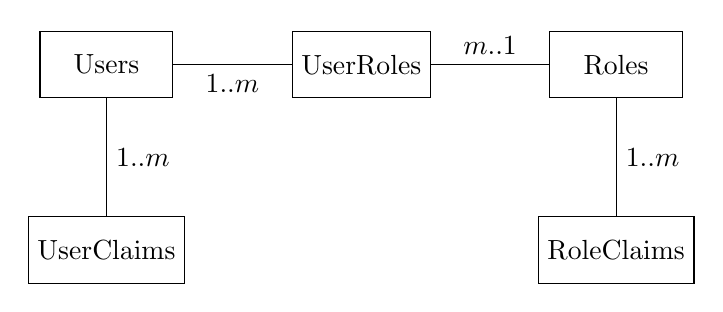
\begin{tikzpicture}[auto,node distance=1.5cm]
\node[entity] (Users) {Users};
\node[entity] (UserRoles) [right = of Users] {UserRoles};
\node[entity] (Roles) [right = of UserRoles] {Roles};
\node[entity] (RoleClaims) [below = of Roles] {RoleClaims};
\node[entity] (UserClaims) [below = of Users] {UserClaims};

\path (UserRoles) edge node {1..\(m\)} (Users) edge node {\(m\)..1} (Roles);
\path (Users) edge node {1..\(m\)} (UserClaims);
\path (Roles) edge node {1..\(m\)} (RoleClaims);
\end{tikzpicture}	
\caption{erd of asp.net identity tables}
\label{fig:asp_net_identity_classes}
\end{figure}

The authorization can be role-based or claim-based. 

The role-based authorization uses checks if the \lstinline|Users| is in a \lstinline|Roles|. To check that simply add the \lstinline|[Authorize(Roles = "RoleName"])]| annotation to a controller method. If the method should be accessible for multiple roles, separate them with a comma: \lstinline|[Authorize(Roles = "Role1,Role2")]|. If more than one role is required, stack the \lstinline|Authrize| Annotations.
\begin{lstlisting}
[Authorize(Roles = "Role1")]
[Authorize(Roles = "Role2")]
public async Task<IActionResult> DoSomething() {...}
\end{lstlisting}
 For an in-depth view about role-based authorization see the official  \href{https://docs.microsoft.com/en-us/aspnet/core/security/authorization/roles}{documentation}.
 
The claim based authorization uses the \lstinline|UserClaims| and \lstinline|RoleClaims| assigned to a user to check if he can access the method.  I will focus on permission based authorization using the Claims. For an in-depth view about claim-based authorization see the official  \href{https://docs.microsoft.com/en-us/aspnet/core/security/authorization/claims}{documentation}.
I added a helper class \lstinline|CustomClaimTypes| very similar to \lstinline|System.Security.Claims.ClaimTypes| with constants
\begin{lstlisting}
public static class CustomClaimTypes
{
	private const string ClaimTypeNamespace = "http://isitar.ch";
	public const string Permission = ClaimTypeNamespace + "/permission";
}
\end{lstlisting}
To keep permissions consistent and easy to manage, I also created the helper class \lstinline|ClaimPermissions| where I store all my permission strings.
\begin{lstlisting}
public static class ClaimPermission
{
	public const string CreateUser = "User.Create";
	public const string DeleteUser = "User.Delete;
	...
}
\end{lstlisting}
To recognize the authorization in a \lstinline|Authorize| annotation I need to configure the Authorization in the \lstinline|ConfigureServices| method in the \lstinline|Startup| class.
\begin{lstlisting}
services.AddAuthorization(options =>
{
	foreach (var prop in typeof(ClaimPermission).GetFields(BindingFlags.Public | BindingFlags.Static | BindingFlags.FlattenHierarchy)
	)
	{
		var propertyValue = prop.GetValue(null).ToString();
		options.AddPolicy(propertyValue, policy => policy.RequireClaim(CustomClaimTypes.Permission, propertyValue));

	}
});
\end{lstlisting}
This adds all the permission claims as a \lstinline|Policy| and it can be checked in the controllers and methods via the \lstinline|Authorize| attribute
\begin{lstlisting}
[Authroize(Policy = ClaimPermission.CreateUser)]
public async Task<IActionResult> DoSomething() {...}
\end{lstlisting}

\subsection{JWT Authentication}
To add JWT support, the Authentiaction needs to be added to the services:

\begin{lstlisting}
services
	.AddAuthentication(config => {
		config.DefaultAuthenticateScheme = JwtBearerDefaults.AuthenticationScheme;
		config.DefaultChallengeScheme =	JwtBearerDefaults.AuthenticationScheme;
	})
	.AddCookie(options => {
		options.SlidingExpiration = true; 
	})
	.AddJwtBearer(JwtBearerDefaults.AuthenticationScheme,
		options =>
		{
			var jwtSettings = Configuration.GetSection("JwtSettings"); 
			options.TokenValidationParameters = new TokenValidationParameters()
			{
				ValidateIssuer = true,
				ValidIssuer = jwtSettings["Issuer"],
				ValidateAudience = true,
				ValidAudience = jwtSettings["Audience"],
				IssuerSigningKey = new SymmetricSecurityKey(
					Encoding.UTF8.GetBytes(jwtSettings["Secret"])
				)
			};
		}
	);
\end{lstlisting}
In the appsettings the following Keys need to be present:
\begin{lstlisting}
"JwtSettings": {
	"Issuer": "isitar.ch",
	"Audience": "DoenerUser",
	"Secret": "SomeVeryLongSecretStringThatIsTotallyRandom"
}
\end{lstlisting}

To generate the JWT-Token a new JwtSecuritytoken needs to be created.
\begin{lstlisting}
[AllowAnonymous]
public async Task<IActionResult> GetTokenAsync([FromBody] LoginViewModel loginViewModel)
{
	if (!ModelState.IsValid)
	{
		return BadRequest(ModelState);
	}
	
	var user = await userManager.FindByNameAsync(loginViewModel.Username);
	var res = await userManager.CheckPasswordAsync(user, loginViewModel.Password);
	if (!res)
	{
		return BadRequest();
	}
	
	var jwtSettings = configuration.GetSection("JwtSettings");
	
	var key = new SymmetricSecurityKey(Encoding.UTF8.GetBytes(jwtSettings["Secret"]));
	var singingCreds = new SigningCredentials(key, SecurityAlgorithms.HmacSha256);
	var expiry = DateTime.UtcNow.AddMinutes(30);
	var claims = await GetValidClaims(user);
	
	var token = new JwtSecurityToken(
		jwtSettings["Issuer"],
		jwtSettings["Audience"],
		claims,
		expires: expiry,
		signingCredentials: singingCreds
	);
	
	return Created("", new
		{
		token = new JwtSecurityTokenHandler().WriteToken(token)
		}
	);
}
\end{lstlisting}
The \lstinline|GetValidClaims| method is explained in \autoref{lst:GetValidClaimsListing} 

\subsection{JWT Authorization}
When authorizing with the JWT-Token, ASP.NET assumes the claims are stored in the token. An easy thing to do is add all claims the user possesses into the token. For this I added a helper method in the \lstinline|LoginController|.
\begin{lstlisting}[label=lst:GetValidClaimsListing]
private async Task<IEnumerable<Claim>> GetValidClaims(User user)
{
	IdentityOptions identityOptions = new IdentityOptions();
	var claims = new List<Claim>
	{
		new Claim(JwtRegisteredClaimNames.Sub, user.UserName),
		new Claim(JwtRegisteredClaimNames.Jti, Guid.NewGuid().ToString()),
		new Claim(JwtRegisteredClaimNames.Iat, DateTimeOffset.UtcNow.ToUnixTimeSeconds().ToString(),
		ClaimValueTypes.Integer64),
		new Claim(identityOptions.ClaimsIdentity.UserIdClaimType, user.Id.ToString()),
		new Claim(identityOptions.ClaimsIdentity.UserNameClaimType, user.UserName),
	};
	var userClaims = await userManager.GetClaimsAsync(user);
	claims.AddRange(userClaims);
	var userRoles = await userManager.GetRolesAsync(user);
	foreach (var userRole in userRoles)
	{
		claims.Add(new Claim(ClaimTypes.Role, userRole));
		var role = await roleManager.FindByNameAsync(userRole);
		if (role != null)
		{
			var roleClaims = await roleManager.GetClaimsAsync(role);
			claims.AddRange(roleClaims);
		}
	}

	return claims;
}
\end{lstlisting}

\section{Swagger}
\subsection{Packages}
\begin{table}
	\centering
	\begin{tabular}{|l l|}
		\hline
		Package & Description \\
		\hline \hline
		Swashbuckle.AspNetcore & For Swagger setup and doc generation \\
		\hline
	\end{tabular}
\end{table}
\subsection{Setup}
To setup the swagger doc the generation needs to be added to the services. 
\begin{lstlisting}
services.AddSwaggerGen(c =>
{
	c.SwaggerDoc("v1", new OpenApiInfo
	{
		Title = "Doener Order Api",
		Version = "v1",
		Description = "Simple doener order app",
	});
}
\end{lstlisting}
The swagger json and swagger ui need to be exposed, so in the \lstinline|Configure| method the following snipped needs to be added 
\begin{lstlisting}
app.UseSwagger();
app.UseSwaggerUI(c =>
{
	c.SwaggerEndpoint("/swagger/v1/swagger.json", "Doener Order Api");
	c.RoutePrefix = "swagger";
});
\end{lstlisting}
With this the swagger ui is accessible under \href{url.tld/swagger}{url.tld/swagger}.

To add the documentation from the methods, the \lstinline|csproj| file needs to be edited so the documentation is exported in an xml file:
\begin{lstlisting}[language=XML]
<PropertyGroup>
	<GenerateDocumentationFile>true</GenerateDocumentationFile>
	<NoWarn>$(NoWarn);1591</NoWarn>
</PropertyGroup>
\end{lstlisting}
The NoWarn removes the warnings for methods that have no documentation. Further the swagger generation (\lstinline|services.AddSwaggerGen|) needs to be extendes by the following snippet:
\begin{lstlisting}
var xmlFile = $"{Assembly.GetExecutingAssembly().GetName().Name}.xml";
var xmlPath = Path.Combine(AppContext.BaseDirectory, xmlFile);
c.IncludeXmlComments(xmlPath);
\end{lstlisting}

To add jwt security to the swagger gen (used to authorize in swagger ui) the following snippet needs to be added in the swagger generation (\lstinline|services.AddSwaggerGen|):
\begin{lstlisting}
c.AddSecurityDefinition("Bearer", new OpenApiSecurityScheme
{
	Description =@"JWT Authorization header using the Bearer scheme. 
		\r\n\r\n Enter 'Bearer' [space] and then your token in the text input below. 
		\r\n\r\nExample: 'Bearer 12345abcdef'",
	Name = "Authorization",
	In = ParameterLocation.Header,
	Type = SecuritySchemeType.ApiKey,
	Scheme = "Bearer",
});
c.AddSecurityRequirement(new OpenApiSecurityRequirement()
{
	{
		new OpenApiSecurityScheme
		{
			Reference = new OpenApiReference
			{
				Type = ReferenceType.SecurityScheme,
				Id = "Bearer"
			},
			Scheme = "oauth2",
			Name = "Bearer",
			In = ParameterLocation.Header,
		},
		new List<string>()
	}
});
\end{lstlisting}

\end{document}
